\subsection*{Practical Details}
A random process can only be observed over a finite span of time.
Consequently, the sample endpoints will typically interrupt any oscillations
at two distinct points in their cycle.
The discrete Fourier transform treats the sample as periodic,
and the resulting discontinuity at the endpoints generates noise,
or \textit{leakage}, in the periodogram.
Smoothing the tails of the sample towards zero,
a process known as \textit{tapering},
eliminates the discontinuity and can help to alleviate leakage.
Following the procedure of Dahlhaus and Janas,
a $10\%$ Tukey-Hanning taper was used for all examples presented here.
Small changes to the taper proportion had little, if any,
effect on the smoothed spectral density estimate $\hat{f}$.
In practice, other tapers can be used with the frequency domain bootstrap.
These were not investigated, to avoid distraction from our focus.

Although tapering reduces noise in the periodogram,
it isn't sufficient to make the periodogram a consistent estimator for the
spectral density.
This requires further smoothing.
In the examples, kernel smoothing is used, with the Epanechnikov kernel
    \[
    K(x) 
    = 
    \frac{3}{4}\pi \biggl[ 1 - \Bigl( \frac{x}{\pi} \Bigr)^2 \biggr].
    \]
Smoothing has a tendency to reduce or eliminate modes of the periodogram,
and care must be taken to preserve important details.
To this end, it's suggested to smooth the log-periodogram rather than smoothing
the periodogram directly.
Further bias correction is possible in light of the distribution of the
periodogram ordinates.
With kernel weights $w_j(x)$ defined in the standard way,
the smoothed, bias-corrected spectral density estimate is given by
    \[
    \hat{f}(x)
    =
    \exp\biggl[
        \sum_{j} w_j(x) \ln I_{j} 
        - \ln \Gamma\bigl(1 + w_j(x)\bigr)
    \biggr],
    \]
where $j = 0, \ldots, \floor{T / 2}$.
The bandwidth is also essential, 
and should be selected to offer a good compromise between noise reduction and
loss of detail.

\subsection*{Example 1}
Consider estimation of the lag-1 autocorrelation $\rho(1)$,
in the $\dist{AR}(1)$ model $X_t = 0.9 X_{t-1} + Z_t$,
using $T = 64$ observations.
The innovations $\{Z_t\}$ are independent and identically distributed
$\dist{U}(-\sqrt{3}, \sqrt{3})$ random variables,
making them a mean 0, variance 1 white noise.
In this setting, the conditions of Theorem~1 are satisfied.
A realization of this process is shown in Figure~\ref{ex1}.
    \begin{figure}[ht]
    \centering
    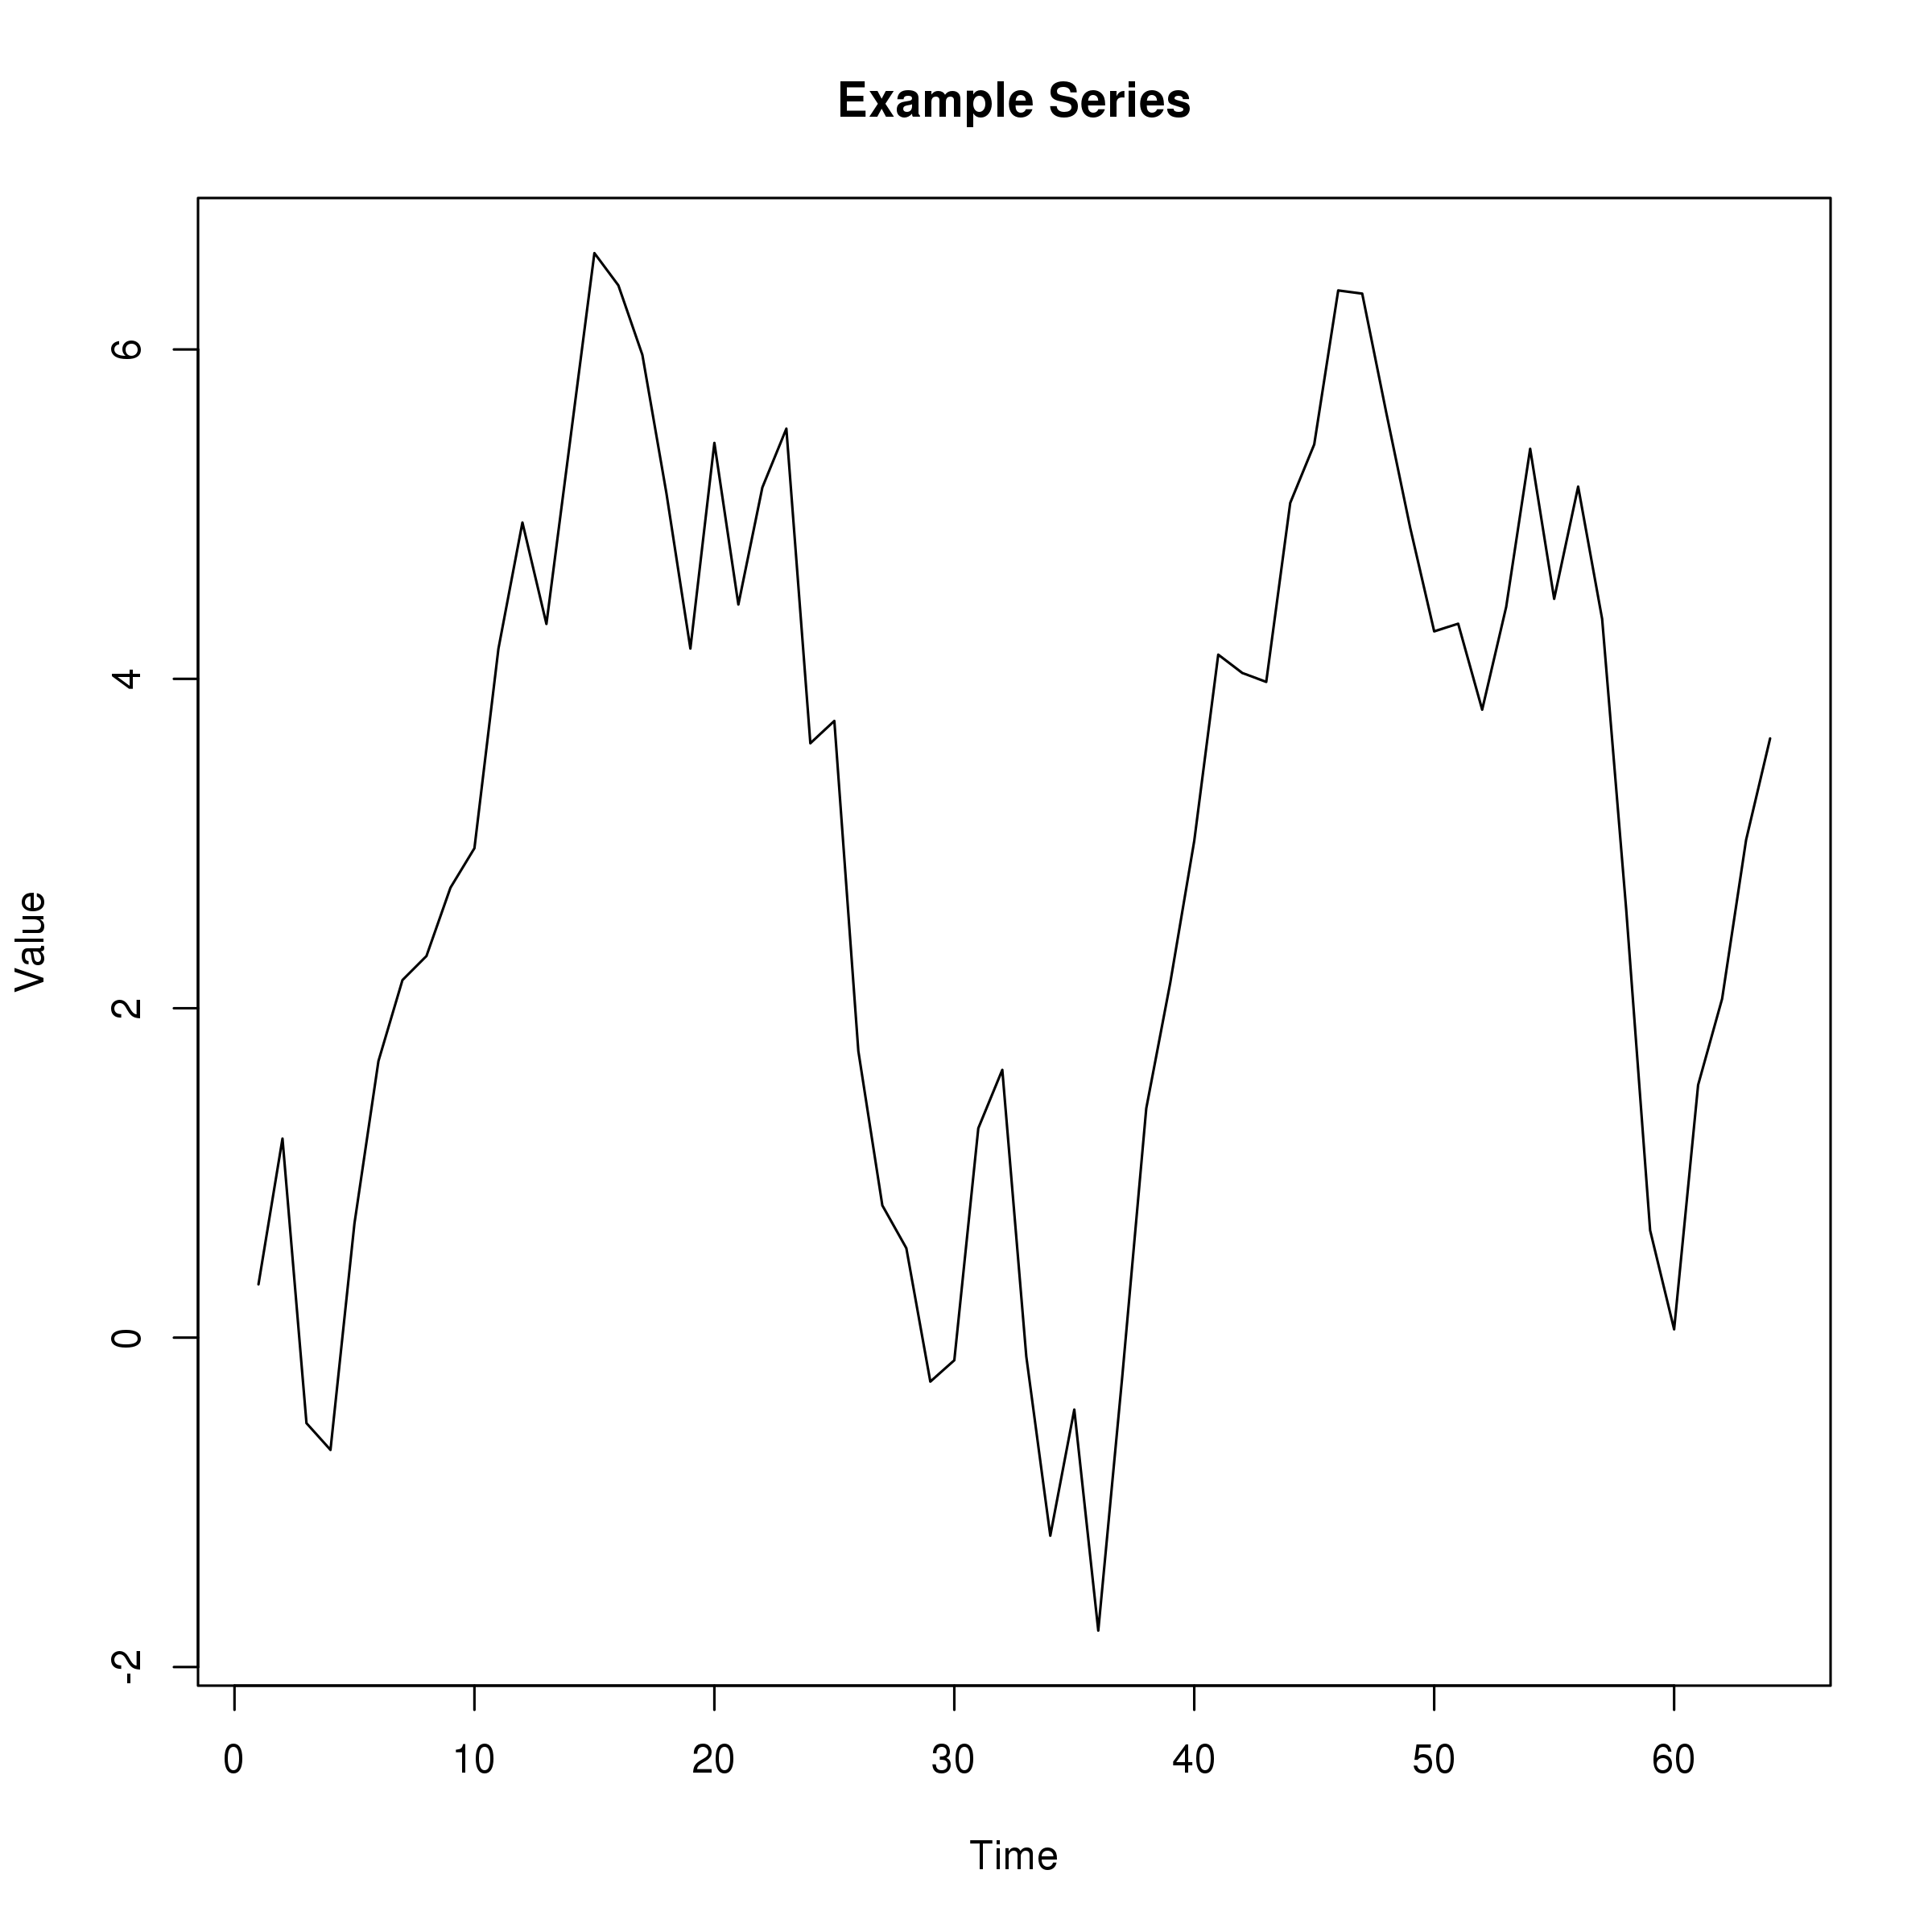
\includegraphics[width = 0.8\textwidth]{../res/ex1.png}
    \caption{
        A realization of the $\dist{AR}(1)$ process in Example 1.
        }
    \label{ex1}
    \end{figure}

A key feature of this model is that its spectral density exhibits a sharp
mode at zero.
This makes spectral density estimation challenging,
because of the trade-offs inherent in smoothing the periodogram.
Figure~\ref{ex1_spec} shows that with a bandwidth of $0.1$,
much of the mode's peak is lost.
On the other hand, reducing the bandwidth to $0.05$ produces a misleading,
bimodal estimate.
The former was selected for use here.
    \begin{figure}[ht]
    \centering
    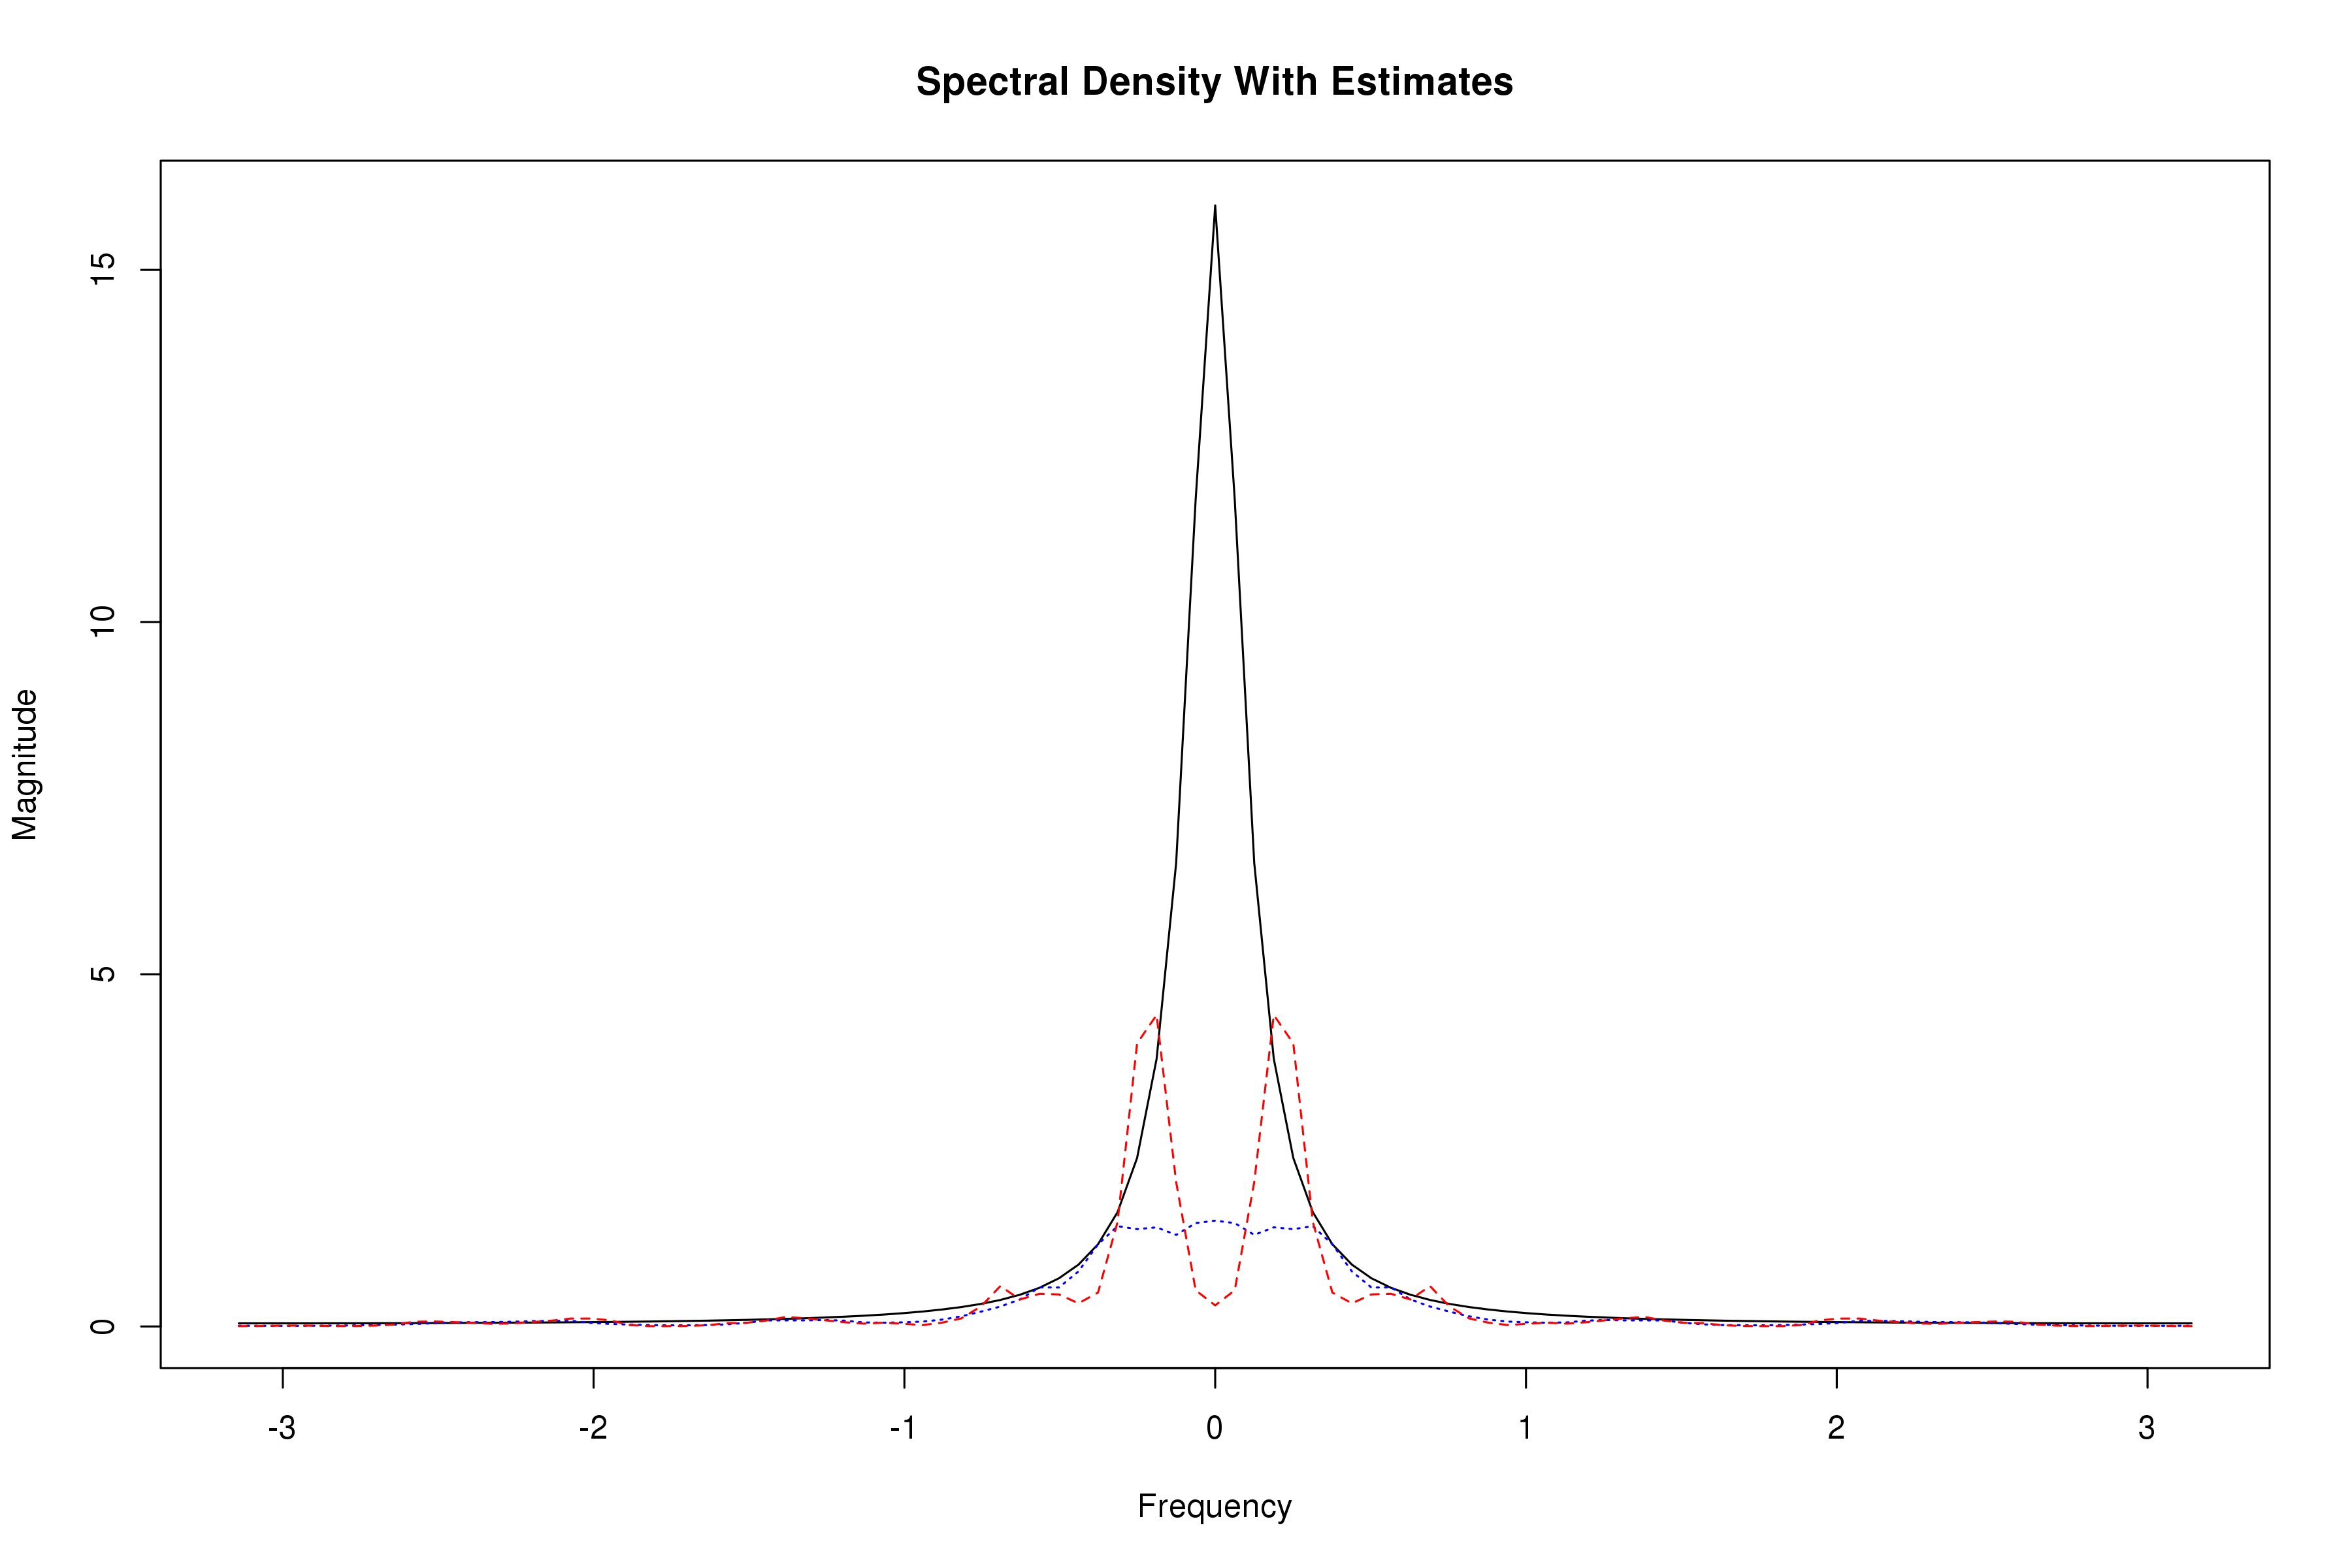
\includegraphics[width = 0.8\textwidth]{../res/ex1_spec.png}
    \caption{
        Example 1
        spectral density (solid, black) and spectral density estimates
        at bandwidth 0.1 (dotted, blue) and 0.05 (dashed, red).
        }
    \label{ex1_spec}
    \end{figure}

The estimate $\hat{\rho}(1)$ for the lag-1 autocorrelation $\rho(1)$
coincides with the Yule-Walker estimate of the AR parameter,
so we have the standard result that as $T \to \infty$,
    \[
        \sqrt{T} \biggl( \frac{\hat{\rho}(1) - 0.9}{c} \biggr)
        \inD
        \dist{N}(0, 1 - 0.9^2),
    \]
where $c$ is a correction for the taper.
This asymptotic error distribution is what would typically be used to construct
confidence bounds on the estimate.
The frequency domain bootstrap provides a bootstrapped error distribution as
a competitor. 
In this case, $2000$ estimates were bootstrapped.
Figure~\ref{ex1_cdf} shows a plot of the cumulative distribution functions for
both, as well as the true distribution (as approximated by repeated 
simulation).
The figure confirms the result of Theorem~1:
the bootstrapped distribution significantly outperforms the asymptotic
distribution.
This result is especially impressive because the spectral density estimate
was not very good---smoothing masked the peak at zero.
Repeated simulations show similarly positive results.
    \begin{figure}[ht]
    \centering
    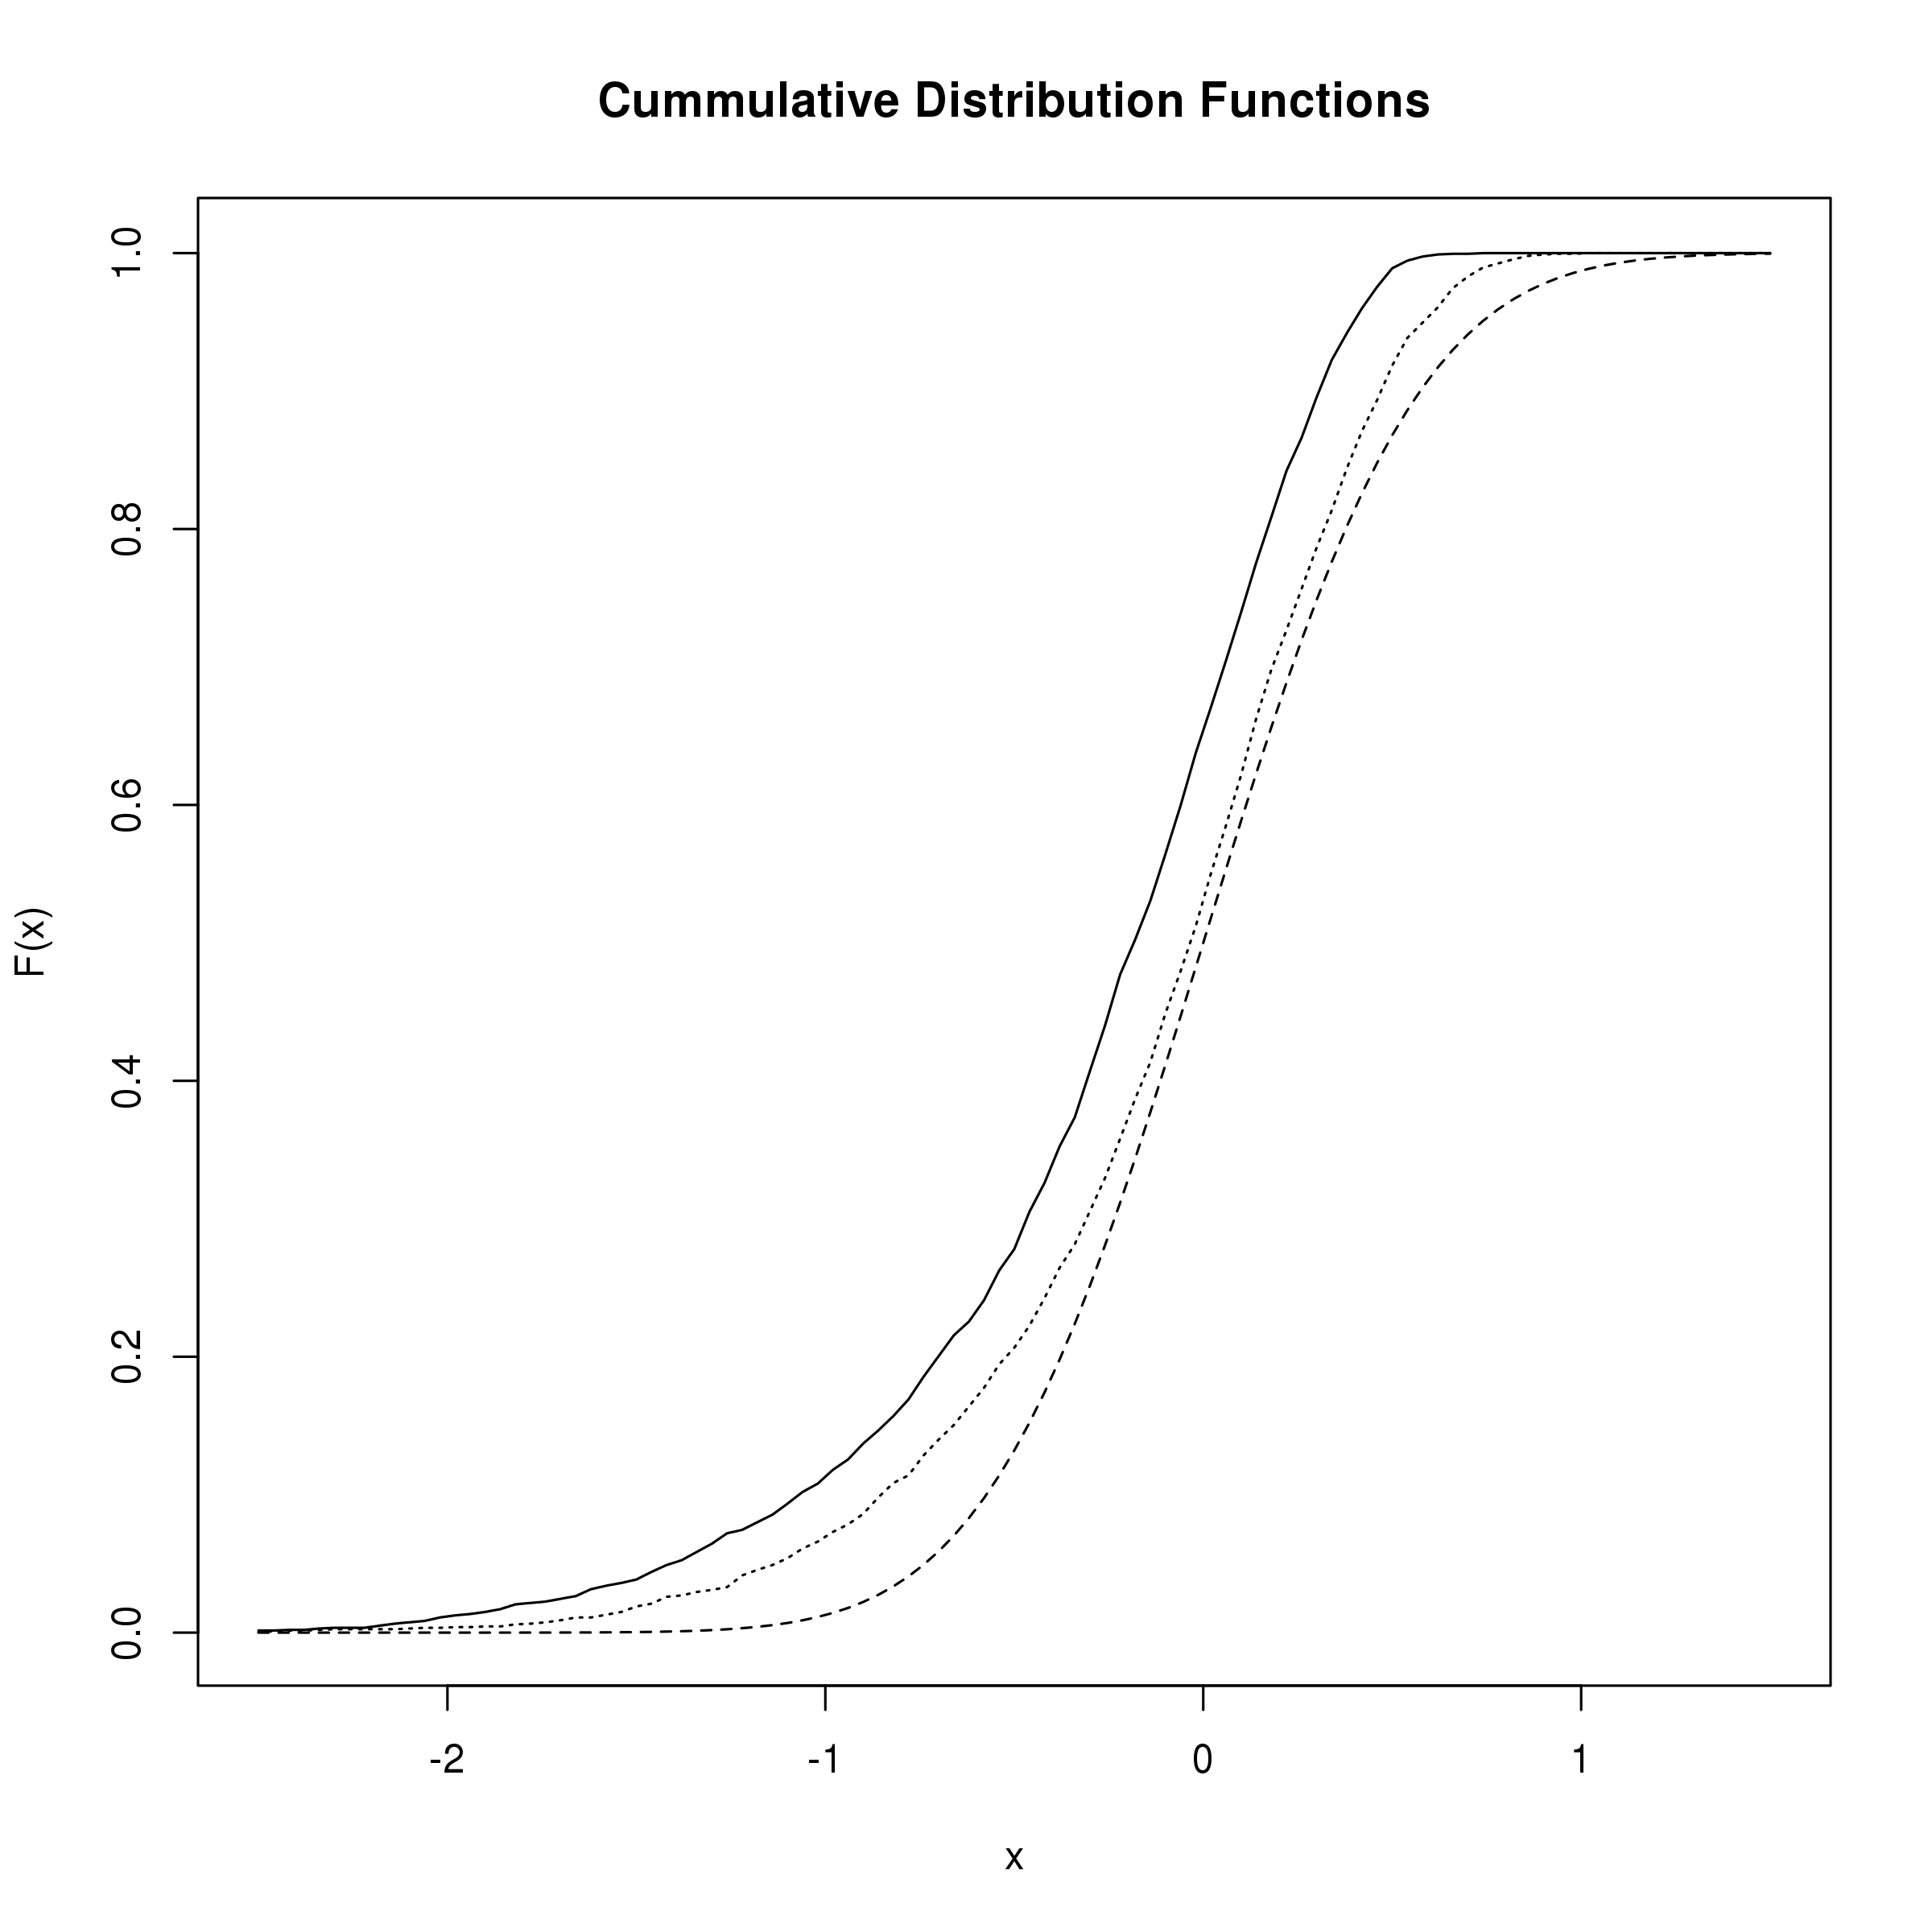
\includegraphics[width = 0.8\textwidth]{../res/ex1_cdf.png}
    \caption{
        Example 1
        CDFs for the true (solid, black), bootstrapped (dotted, blue),
        and asymptotic (dashed, red) error distributions.
        }
    \label{ex1_cdf}
    \end{figure}

\subsection*{Application}
    \begin{figure}[ht]
    \centering
    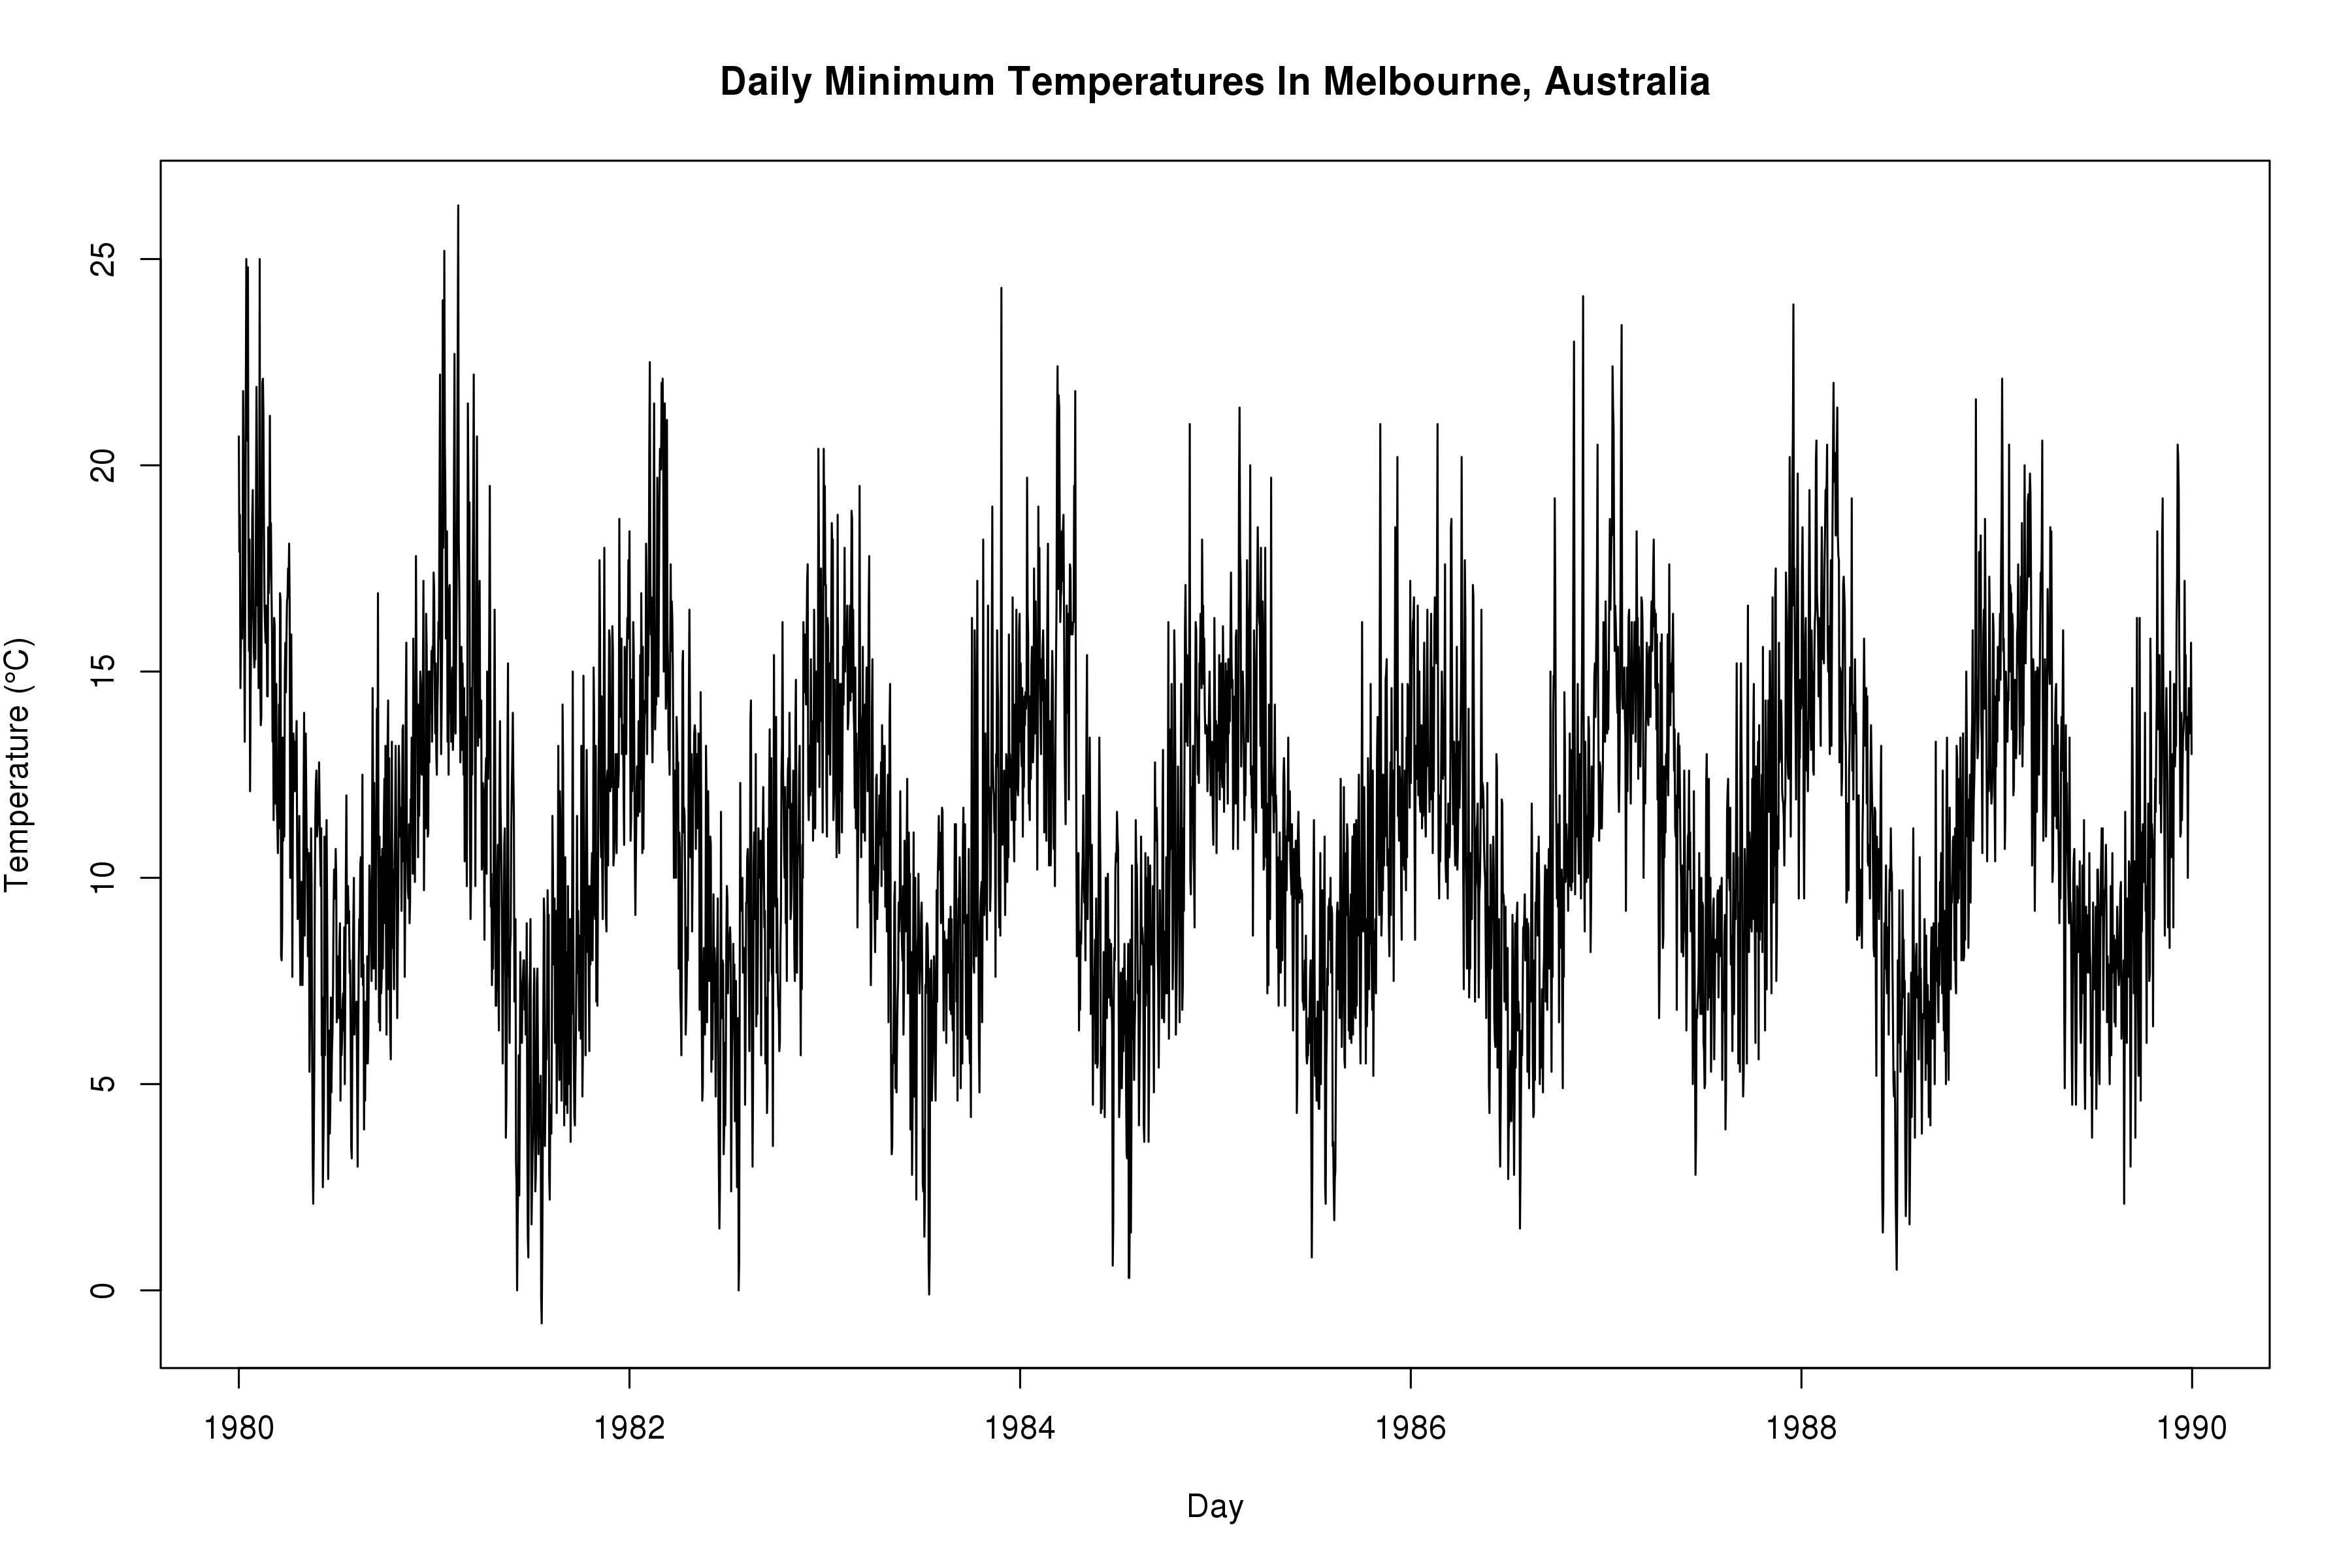
\includegraphics[width = 0.8\textwidth]{../res/exA.png}
    \caption{
        The Melbourne temperatures time series used in the application.
        }
    \label{ex1_cdf}
    \end{figure}
